\documentclass[preprint]{aastex}
%\documentclass[aps,prd,preprint,showpacs,superscriptaddress,amsmath]{revtex4}
%\documentclass[prd,showpacs,superscriptaddress,twocolumn,
%floatfix,preprintnumbers,altaffilletter]{revtex4}
%\documentclass[prd,showpacs,superscriptaddress,
%floatfix,preprintnumbers,altaffilletter]{revtex4}

\usepackage{longtable}
\usepackage{graphicx}
\usepackage{amsmath,amssymb}
\usepackage{color}
\usepackage{units}
\usepackage{epstopdf}
\usepackage{hyperref}
\usepackage{multirow}

\usepackage{tikz}
\usetikzlibrary{shapes,arrows}

\usepackage{listings}
\usepackage{color}

\definecolor{dkgreen}{rgb}{0,0.6,0}
\definecolor{gray}{rgb}{0.5,0.5,0.5}
\definecolor{mauve}{rgb}{0.58,0,0.82}

\lstset{frame=tb,
  language=python,
  aboveskip=3mm,
  belowskip=3mm,
  showstringspaces=false,
  columns=flexible,
  basicstyle={\small\ttfamily},
  numbers=none,
  numberstyle=\tiny\color{gray},
  keywordstyle=\color{blue},
  commentstyle=\color{dkgreen},
  stringstyle=\color{mauve},
  breaklines=true,
  breakatwhitespace=true,
  tabsize=3
}

%\usepackage[doublespacing]{setspace}

\newcommand{\braket}[2]{\left\langle#1\, |\,#2\,\right\rangle}  %  < #1 | #2 >
\newcommand{\expec}[1]{\langle#1\rangle}  %  < #1 >
\newcommand{\drm}{{\rm d}}
\newcommand{\irm}{{\rm i}}
\newcommand{\beq}{\begin{equation}}
\newcommand{\eeq}{\end{equation}}
\newcommand{\bdm}{\begin{displaymath}}
\newcommand{\edm}{\end{displaymath}}
\newcommand{\T}[1]{\tilde{#1}}
\newcommand{\wT}[1]{\widetilde{#1}}
\newcommand{\Cdot}{\!\cdot\!}
\newcommand{\SNR}{\textnormal{SNR}}
\newcommand{\rednote}[1]{{\color{red} (#1)}}
\definecolor{Gray}{gray}{0.9}
\definecolor{orange}{rgb}{0.9,0.5,0}
\newcommand{\td}[1]{{\textcolor{orange}{\texttt{TD: #1}} }}

\graphicspath{{./plots/}}
\begin{document}

%\pacs{95.75.-z,04.30.-w}

\title{gwemopt: Optimizing searches for electromagnetic counterparts of gravitational wave triggers}

\author{Man Leong Chan}
\affil{University of Glasgow, Glasgow G12 8QQ, United Kingdom}

\author{Deep Chatterjee}
\affil{University of Wisconsin-Milwaukee, Milwaukee, WI 53201, USA}

\author{Michael Coughlin}
\affil{Department of Physics, Harvard University, Cambridge, MA 02138, USA}

\author{Shaon Ghosh}
\affil{University of Wisconsin-Milwaukee, Milwaukee, WI 53201, USA}

\author{Giuseppe Greco}
\affil{INFN, Sezione di Firenze, I-50019 Sesto Fiorentino, Firenze, Italy}

\author{Yiming Hu}
\affil{TianQin Research Center for Gravitational Physics, Sun Yat-sen University, Tangjiawan, Zhuhai 519082, Guangdong, P. R. China}

\author{Shasvath Kapadia}
\affil{University of Wisconsin-Milwaukee, Milwaukee, WI 53201, USA}

\author{Javed Rana}
\affil{Inter-University Centre for Astronomy and Astrophysics, Pune 411007, India}

\author{Om Sharan Salafia}
\affil{INAF - Osservatorio Astronomico di Brera Merate, via E. Bianchi 46, I–23807 Merate, Italy}

\author{Duo Tao}
\affil{Carleton College, Northfield, MN 55057, USA}

\begin{abstract}

Documentation for gwemopt

\end{abstract}

\maketitle

\section{Introduction}
\label{sec:Intro}

There has been significant effort expended in the search for the electromagnetic counterpart of the gravitational waves found by compact binary black hole systems \citep{AbEA2016a,AbEA2016g,AbEA2017}.
In general, there is significant optimism for the potential counterparts for emission from binary neutron star and black hole - neutron star systems across timescales and wavelengths \citep{Nakar2007,MeBe2012}. 

To facilitate the detection of gravitational-wave counterparts, probability skymaps as a function of sky direction and distance are released for gravitational wave triggers produced by the detectors \citep{SiPr2014,BeMa2015}. 
Due to the significant sky coverage required to observe the gravitational-wave sky localization regions, usually spanning $\approx 100\,\textrm{deg}^2$, techniques to optimize the followup efforts are of significant utility \citep{Fair2009,Fair2011,Grover:2013,WeCh2010,SiAy2014,SiPr2014,BeMa2015,EsVi2015,CoLi2015,KlVe2016}.
Given the large sky localization regions involved, wide-field survey telescopes have the best opportunities to make a detection. 
The Panoramic Survey Telescope and Rapid Response System (Pan-STARRS) \cite{MoKa2012}, Asteroid Terrestrial-impact Last Alert System (ATLAS) \cite{Ton2011}, the intermediate Palomar Transient Factory (PTF) \cite{RaSh2009} and (what will become) the Zwicky Transient Facility (ZTF), BlackGEM \cite{BlGr2015} and the Large Synoptic Survey Telescope (LSST) \cite{Ivezic2014} are all examples of such systems.
For example, Pan-STARRS has a 7$^\circ$ field of view (FOV), achieving a 5 $\sigma$ limit of 21.5 (AB mag) in the i band in a 45 second exposure. ATLAS has a 29.2$^\circ$ field of view, achieving a 5 $\sigma$ limit of 18.7 in the cyan band in a 30 second exposure. For comparison, LSST will have a $9.6\textrm{deg}^2$ FOV and will require a 21\,s r-band exposure length to reach 22 mag.

Due to the significant difference in telescope configurations, including FOV, filter, typical exposure times, and limiting magnitudes, in addition to placement on the earth and therefore different seeing and sky conditions, optimizing gravitational wave followups for generic telescopes is difficult. Therefore, in the following, we will take Pan-STARRS and ATLAS as examples. Although the question of optimizing multiple telescope coordination has been explored previously, these concentrated on tiling the sky in an optimal way in order to limit overlapping images \citep{SiPr2012}. Due to the practical difficulties in coordinating telescopes at that level, which generally requires the coordination of multiple teams and sites, we will focus on how multiple telescopes can allocate their time across the likelihood region in order to maximize the number of transients detected.

For this reason, we have created a codebase named \emph{gwemopt} that utilizes methods from a variety of recent papers geared towards optimizing efforts of followup. We employ methods to read gravitational-wave skymaps and the associated information made available from GraceDB \footnote{https://gracedb.ligo.org}, in addition to information about the telescopes to tile the sky, allocate available telescope time to the chosen fields, and schedule that time in a way that optimizes based on expected lightcurves.
In section~\ref{sec:algorithm}, we describe the algorithm.
In section~\ref{sec:performance}, we describe the performance of the algorithms.
In section~\ref{sec:conclusions}, we offer concluding remarks and suggest directions for future research.

\section{Algorithm}
\label{sec:algorithm}

Figure~\ref{fig:flowchart} shows the flowchart for the \emph{gwemopt} pipeline, developed to optimize the efforts of electromagnetic followup of gravitational-wave events.
It uses events provided by gracedb in addition to information about the telescopes to creating tiles and optimize time allocations in the fields.
It uses information about potential lightcurves from electromagnetic counterparts to schedule the available telescope time.

% Define block styles
\tikzstyle{decision} = [diamond, draw, fill=blue!20,
    text width=4.5em, text badly centered, node distance=3cm, inner sep=0pt]
\tikzstyle{block} = [rectangle, draw, fill=blue!20,
    text width=5em, text centered, rounded corners, minimum height=3em]
\tikzstyle{line} = [draw, -latex']
\tikzstyle{cloud} = [draw, ellipse,fill=red!20, node distance=3cm,
    minimum height=2em]
\tikzstyle{emptyblock} = [rectangle, minimum height=3em]

\begin{figure}[t]
 \begin{center}
 \begin{tikzpicture}[node distance = 2.3cm, auto]
    % Place nodes
    \node [emptyblock] (init) {};
    \node [block, left of=init] (GraceDB) {GraceDB};
    \node [block, right of=init] (Telescope) {Telescope};
    \node [block, below of=init] (Tiling) {Tiling of the field of view};
    \node [block, below of=Tiling] (Time) {Calculate time allocations};
    \node [block, below of=Time] (Schedule) {Schedule observations};
    \node [block, below of=Schedule] (Efficiency) {Calculate efficiencies};
    % Draw edges
    \path [line] (GraceDB) -- (Tiling);
    \path [line] (Telescope) -- (Tiling);
    \path [line] (Tiling) -- (Time);
    \path [line] (Time) -- (Schedule);
    \path [line] (Schedule) -- (Efficiency);
 \end{tikzpicture}
 \end{center}
 \caption{A flow chart of the \emph{gwemopt} pipeline.}
 \label{fig:flowchart}
\end{figure}

\subsection{GraceDB}

\begin{figure}[t]
\hspace*{-0.5cm}
\centering
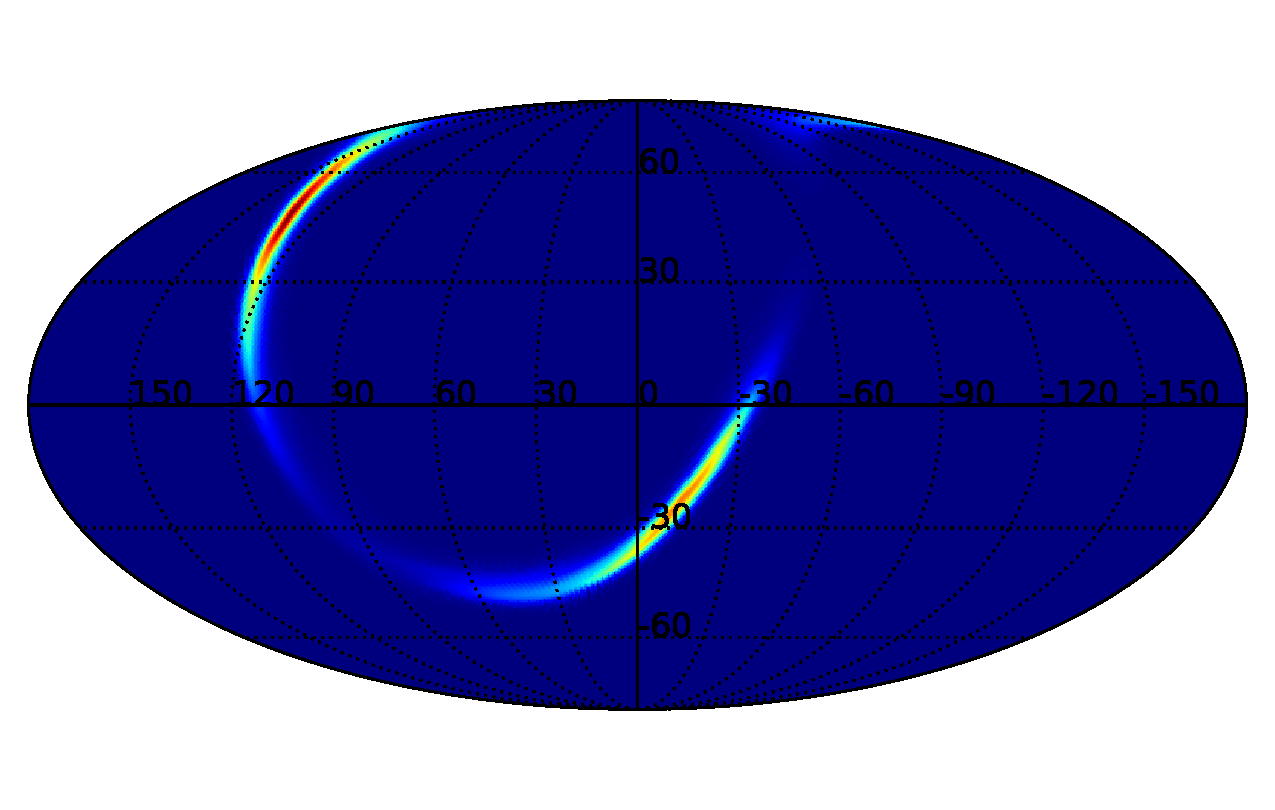
\includegraphics[width=4in]{prob.pdf}
\caption{The gravitational-wave likelihood $L_\textrm{GW}(\alpha,\delta,R)$ for GW170104.}
 \label{fig:skymap}
 \end{figure}

\begin{lstlisting}
python gwemopt_run --doEvent --do3D --event G268556
\end{lstlisting}

The gravitational-wave candidate event database (GraceDB) is a service that provides information on candidate gravitational-wave events and the multi-messenger followups performed on them. An API is made available that allows for access to this information.
\emph{gwemopt} uses this API to access information pertinent for gravitational-wave followups.
First of all, it downloads the gravitational-wave skymap for a given event; an example is shown in figure~\ref{fig:skymap}.
In addition, information such as the time of the event, the time delay between the time-of-arrival at the detectors, and \rednote{EM bright} information is noted.

\subsection{Telescope configuration}

We require standardized configuration files for the telescopes to be analyzed. 
The information includes the filter being used, the limiting magnitude of the instrument and the exposure time required to achieve that magnitude, site location information, and information about the field of view shape and size. For the field of view, two options, square and circle are available, with the FOV being specified by the length of the square side and the radius of the circle. In addition, a tesselationFile is requested. This is especially useful for telescopes such as ZTF which use fixed telescope pointings which ensures the availability of reference images. In case a tesselation file is not available, one is automatically generated, described in the next section.
Configuration files for ATLAS, BlackGEM, LSST, PS1, and ZTF are available.

\begin{lstlisting}
filter c
magnitude 18.7
exposuretime 30.0
latitude 20.7204
longitude -156.1552
elevation 3055.0
FOV_coverage 5.46
FOV 5.46
FOV_coverage_type square
FOV_type square
tesselationFile ../input/ATLAS.tess
\end{lstlisting}

\subsection{Skymap tiling}

There are four options related to skymap tiling currently available, moc, ranked, hierarchical and greedy.

\emph{moc}. Multi-order coverage of healpix maps hierarchically predefines cells in order to specify arbitrary sky regions \cite{FeBo2014}.

\emph{ranked}. Ghosh et al. \cite{GhBl2016} use pre-defined sky cells...

\emph{hierarchical}. A Multinest based optimization which optimizes tiles for a given skymap by placing them sequentially.

\emph{greedy}. An emcee based optimization which optimizes tiles for a given skymap by placing them simultaneously.

\subsection{Time allocations}

There are four options related to time allocations as a function of sky location available, powerlaw, WAW, PEM, and coverage.

\emph{Powerlaw.} Coughlin and Stubbs \cite{CoSt2016} derived scaling relations for the time allocated to any given field, $t_i$, given the graviational-wave likelihood. We showed that under certain assumptions, $t_i \propto \left(\frac{L_\textrm{GW}(\alpha_i,\delta_i)}{a(\alpha_i,\delta_i)}\right)^{2/3}$, where $L_\textrm{GW}(\alpha_i,\delta_i)$ is the gravitational-wave likelihood and $a(\alpha_i,\delta_i)$ is Galactic extinction. 

\emph{WAW (Where and when).} Salafia et al. \cite{SoCo2017} use counterpart lightcurve models in the optical, infrared and radio constructed from information from the gravitational-wave signals to create a time- and sky location dependent probability for detecting electromagnetic transients.

\emph{PEM (Probability of electomagnetic counterpart).} Chan et al. \cite{ChHu2017} optimize the number of fields to observe and their time allocations by adopting priors on the intrinsic luminosity of the sources and using knowledge of distance to the counterparts provided for compact binary coalescence.

\emph{Coverage.} This is an option whereby coverage from existing surveys, including the right ascension and declination of the pointing and the limiting magnitude, are used.

\subsection{Scheduling}

There are three options related to scheduling observations, greedy, sear, and weighted.

\emph{Greedy.} Rana et al. \cite{RaSi2017} implemented a greedy algorithm whereby the field with the highest probability region in a given time window is observed. As this analysis did not include the possibility of multiple exposures for each pointing, it is modified in the analysis to include multiple exposures. The algorithm is as follows:

\begin{enumerate}
\item Construct a list of the tiles and number of exposures for each tile based on the time allocation algorithm utilized.
\item For each window, find the sky tiles that are in the current window: $T_0 + (j-1) T_{exp}$ and $T_0 + j T_{exp}$
\item Allocate the window to the sky tile with the greatest probability, and increment the number of exposures for that tile down by 1.
\end{enumerate}

\emph{sear (Setting Array).} Rana et al. \cite{RaSi2017} also implemented a version whereby the rising and setting of tiles were accounted for. It uses the idea that observes high probability tiles first, subject to the condition that each tile from the
observing sequence must be observed before it sets.

\emph{weighted.} Given the impossibility of necessarily observing all of the tiles as they rise and set given the requirement of using multiple exposures per tile, we are motivated to define a scheme whereby each tile is given a weight based on both gravitational-wave likelihood enclosed, the number of exposures required for that tile, and the number of available slots for it to be image. Therefore we define the weights $w_i$ as

\begin{equation}
w_i = L_\textrm{GW}(\alpha_i,\delta_i) \times \frac{N_\textrm{R}}{N_\textrm{A}} 
\end{equation}

\subsection{Efficiency}

To estimate the efficiency for the ``detection'' of the electromagnetic counterparts to gravitational-wave transients, we perform simulated injections of supplied lightcurves. We provide example lightcurves for a variety of lightcurve models, including:

\begin{enumerate}
\item Tanaka et al. \cite{TaHo2014}: Simulations of binary systems showing ejecta morphology and resulting lightcurves.
These simulations led to analytical models for black-hole neutron star systems from \item Kawaguchi et al. \cite{KaKy2016}: Analytical models for black-hole neutron star systems based on Tanaka et al. \cite{TaHo2014}
\item Dietrich and Ujevic \cite{DiUj2017}: Analytical models for binary neutron star systems based on Tanaka et al. \cite{TaHo2014}
\item Barnes et al. \cite{BaKa2016}: Simulations of binary systems studying the emission profiles of radioactive decay products from the merger.
\item Metzger et al. \cite{MeBa2015}: Blue ``precursor'' to the kilonovae driven by $\beta$-decay of the ejecta mass.
\end{enumerate}

The requirements for ``detection'' of the electromagnetic counterparts to gravitational-wave transients are as follows.
We require that the transient appear in \rednote{?} images over \rednote{?} nights.
In each image, the transient must exceed the limiting magnitude in that image.
The color of the transient is estimated from the filter given in the configuration file.
We simulate the transients at a variety of location and distances consistent with the gravitational-wave probability skymap.


\section{Performance}
\label{sec:performance}

\section{Conclusion}
\label{sec:conclusions}

\section{Acknowledgments}
MC is supported by National Science Foundation Graduate Research Fellowship Program, under NSF grant number DGE 1144152.

\bibliographystyle{plainnat}
\bibliography{references}

\end{document} 
